\documentclass{beamer}
\usetheme{Madrid}

\usepackage{amsmath, amssymb, amsthm}
\usepackage{graphicx}
\usepackage{listings}
\usepackage{gensymb}
\usepackage{minted}
\usemintedstyle{friendly}
\definecolor{bg}{rgb}{0.95,0.95,0.95}
\usepackage[utf8]{inputenc}
\usepackage{hyperref}
\usepackage{gvv}
\begin{document}
\title{NCERT 10.4.EX1}
\author{EE24BTECH11032 - JOHN BOBBY}
\date{}
\frame{\titlepage}
\begin{frame}{Question}
\textbf{Alex and Sam together have 45 marbles. Both of them lost 5 marbles each, and the product of the number of marbles they have is 124. Find how many marbles they had at the beginning.}
\end{frame}
\begin{frame}{Quadratic Formula}
Let  the number of marbles Alex have at the beginning$=x$\\
The number of marbles Sam have $=45-x$\\
After losing $5$ marbles,\\
Number of marbles alex has $x-5$\\
Sam now has $45-x-5=50-x$\\
Product of marbles $=124$\\
$\brak{x-5}\brak{50-x}=124$\\
On rearranging,\\
$x^2-45x+324=0$\\
\begin{align*}
    x &= \frac{-b \pm \sqrt{b^2 - 4ac}}{2a}  \\ 
    x=9\text{ or }36
\end{align*}
\end{frame}
\begin{frame}{Eigen Value Method}
    For a quadratic equation $ax^2+bx+c$ the roots are the eigen values of the companion matrix \\
    $$\myvec{0 & 1\\ \frac{-c}{a} & \frac{-b}{a}}=\myvec{ 0 & 1 \\-324 & 45}$$
    We can apply the QR algorithm to find the eigen values of this matrix\\
    Using Gram-Schmidt alogorithm  the matrix $\vec{A}$ can be factorised as \\
    \begin{align*}
        \vec{A}=\vec{QR}
    \end{align*}
    Where $\vec{Q}$ is a orthogonal matrix and $\vec{R}$ is a upper triangular matrix.\\
    The process continues in the following manner
    \begin{align*}
        \vec{A_k}=\vec{Q_kR_k}\\
        \vec{A_{k+1}}=\vec{R_kQ_k}
    \end{align*}
    For large values of $k$ the diagonal elements of the  matrix $\vec{A_k}$ converges to the eigen values. 
\end{frame}
\begin{frame}{Newton-Raphson Method}
\begin{enumerate}
    \item Choose a starting point $x_0$ which is close to a root
    \item Update the value of $x$ accordingly,\\
     $$x_{n+1}=x_n-\frac{f\brak{x}}{f^\prime\brak{x}}$$\\
     $$x_{n+1} &= x_{n} - \frac{x_{n}^2 - 45x_{n} + 324}{2 x_{n} - 45}$$
     \item The value of $x$ will converge to one of the roots
\end{enumerate} 
\end{frame}
\begin{frame}[fragile]
\frametitle{C-Code}
\begin{minted}[bgcolor=bg, linenos, fontsize=\scriptsize, breaklines]{c}
#include <stdio.h>
#include <math.h>
#define EPSILON 0.000001 
void function(double *x,double *y,int n){
	for(int i=0;i<n;i++)
	y[i]=x[i]*x[i]-45*x[i]+324;
}
double f(double x) {
    return x * x - 45 * x + 324;
}
double f_prime(double x) {
    return 2 * x - 45;
}
double NR(double guess1){
    double x0, root;
    x0=guess1;int iteration = 0;
    while (1) {
        double fx = f(x0);
        double fx_prime = f_prime(x0);
        root = x0 - fx / fx_prime;
        printf("Iteration %d: x = %.6f\n", iteration + 1, root);
        if (fabs(root - x0) < EPSILON)
        break;
        x0 = root;
        iteration++;
    }
    return root;
}
\end{minted}
\end{frame}
\begin{frame}[fragile]
\frametitle{Python-Code}
\begin{minted}[bgcolor=bg, linenos, fontsize=\scriptsize, breaklines]{python}
import numpy as np
import matplotlib.pyplot as plt
import ctypes
# Load the shared library
lib = ctypes.CDLL('./lib.so')
lib.function.argtypes=[ctypes.POINTER(ctypes.c_double), ctypes.POINTER(ctypes.c_double), ctypes.c_int]
lib.f.argtypes=[ctypes.c_double]
lib.f.restype=ctypes.c_double
lib.f_prime.argtypes=[ctypes.c_double]
lib.f_prime.restype=ctypes.c_double
lib.NR.argtypes = [ctypes.c_double]
lib.NR.restype = ctypes.c_double
# Parameters
x_start = 0
x_end = 40
h = 0.1
n_steps = 401
x = np.linspace(x_start, x_end, n_steps)
y = np.zeros(n_steps)
\end{minted}
\end{frame}

\begin{frame}[fragile]
\frametitle{Python-Code}
\begin{minted}[bgcolor=bg, linenos, fontsize=\scriptsize, breaklines]{python}
# Conversion to ctypes array
x_ctypes = x.ctypes.data_as(ctypes.POINTER(ctypes.c_double))
y_ctypes = y.ctypes.data_as(ctypes.POINTER(ctypes.c_double))
lib.function(x_ctypes, y_ctypes, n_steps)
root1=lib.NR(5)
root2=lib.NR(25)
# Plotting
plt.figure(figsize=(10, 6))
plt.plot(x, y, label="Theory", linestyle='-', color='b', linewidth=5)
plt.scatter(root1, 0, color='r', marker='o', s=100, zorder=5, label=f"Root at x={root1:.2f}")
plt.scatter(root2, 0, color='r', marker='o', s=100, zorder=5, label=f"Root at x={root2:.2f}")
plt.xlabel("x")
plt.ylabel("y")
plt.legend(['f(x)=$x^2-45x+324$',f"Root at x={root2:.2f}",f"Root at x={root1:.2f}"])
plt.grid()
plt.savefig('plot.png')
\end{minted}
\end{frame}
\begin{frame}{Plot}
    \begin{figure}[h]
\centering
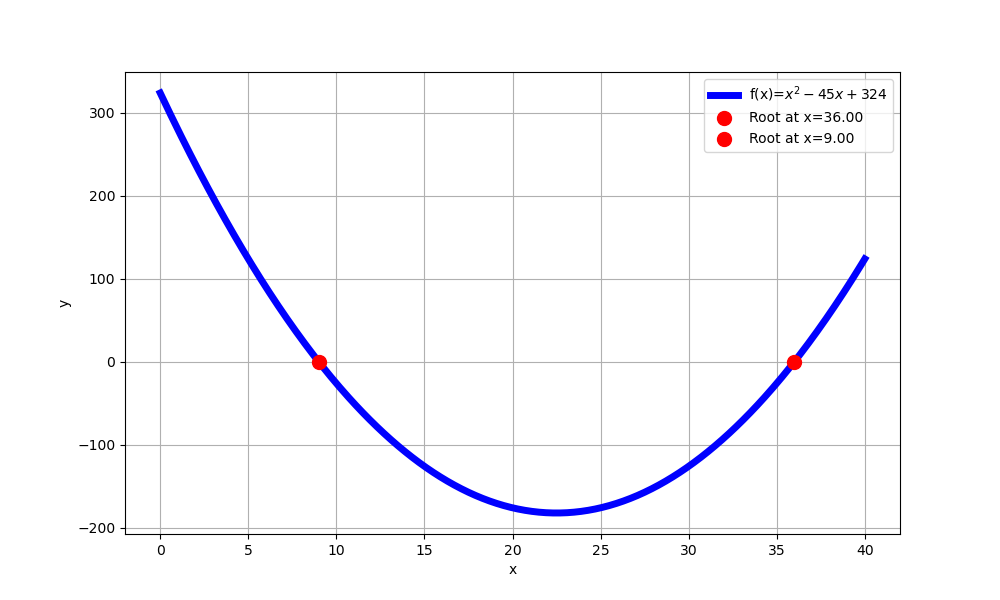
\includegraphics[width=\columnwidth]{figs/Q5.png}
\caption{Plot using Newton-Raphson method}
\label{fig:Plot1} 
\end{figure}
\end{frame}

\end{document}

